\section{Introduction}

Although the traditional relational data model has been the preferred choice for data representation for decades, the advent of Big Data has exposed its limitations in various aspects. Many technologies and approaches considered mature and sufficiently robust have reached their limits when applied to Big Data. One of the most daunting challenges is the \textit{variety} of data, which encompasses multiple types and formats that originate from diverse sources and are inherently adherent to different models. There are structured, semi-structured, and unstructured formats; order-preserving and order-ignorant models; aggregate-ignorant and aggregate-oriented systems; models where data normalization is critical or the redundancy is naturally supported; etc.

The naturally contradictory features of the so-called \textit{multi-model data} introduce an additional dimension of complexity to all aspects of data management, including modelling, storing, querying, transforming, integrating, updating, indexing, and many more. Hence, several multi-model tools for data management have emerged. For example, considering the storage of multi-model data, more than 2/3 of the 50 most widely used database management systems (DBMSs)\footnote{\url{https://db-engines.com/en/ranking}} now fall under the category of \textit{multi-model} following the Gartner prediction~\citep{Gartner2015} made almost 10 years ago. Unfortunately, no standards exist on which models to combine and how, so each DBMS provides a proprietary solution.

Similarly, there exist \textit{polystores}~\citep{conf/cikm/LuHC18,DBLP:journals/ijcc/BondiombouyV16}, sometimes denoted as \textit{multi-database systems}. The general idea is that several distinct data management systems (usually single-model) live under a common, integrated schema provided to the user. Polystores can be further classified~\citep{conf/bigdataconf/TanCGM17} depending on various aspects, such as the number of query interfaces or the types of underlying systems (homogeneous or heterogeneous), the level of autonomy of the underlying systems, etc. So, again, the variety of choices is wide.

% Also, the number of query languages reflects the situation of the existing systems when considering the multi-model data. Despite being primarily denoted for the relational model, numerous SQL-like languages are currently used for various other models and their combinations. For instance, the Cassandra Query Language (CQL)\footnote{\url{https://cassandra.apache.org/doc/stable/cassandra/cql/}} is an SQL-like query language in column-family DBMS Apache Cassandra. Or, the Array Query Language (AQL)\footnote{\url{https://www.nersc.gov/assets/Uploads/scidb-userguide-12.3.pdf}}, also SQL-like, is used in array DBMS SciDB to query multi-dimensional arrays. And SQL has also been extended to support cross-model querying. Apart from numerous proprietary solutions~\citep{CSUR-Jiaheng}, there are also two ISO standards for querying relational and document data -- SQL/XML~\citep{SQLXML} and SQL/JSON~\citep{SQLJSON}. In general, an extensive overview of existing multi-model query languages (developed within various DBMSs) is provided in a recent survey~\citep{Jiaheng2023Survey}. %The authors classify the approaches into SQL extensions, XPath/XQuery extensions, graph query extensions, and also several native multi-model languages. 

Choosing the optimal tool for the particular use case is highly challenging, considering the range of each area's approaches. Naturally, we need to be able to compare the selected set of tools for \textit{all} target use cases, and benchmarking comes into play. Despite many single-model benchmarks and data generators for all the common models (see Section~\pRef{sec:rel}), the shift to the multi-model world is not straightforward. The multi-model test cases must cover the required subset of models and their mutual relations, such as multi-model embedding, cross-model references, or multi-model redundancy. In addition, the variety of use cases grows with the number of distinct models combined. Hence, the number of truly multi-model benchmarks is small, and their versatility and coverage are limited.

In response to this problem, we propose a solution that enables the creation of virtually any possible multi-model data set together with the respective operations. To ensure the data sets have realistic characteristics, we do not utilize the classical approach of exploitation of generators, providing values with a required distribution. Instead, this paper proposes a framework for transforming given single- (or multi-) model data and queries to any possible combination of multi-model data and queries.

Our approach is based on utilizing the toolset we have developed in our research group for various aspects of multi-model data management based on the unifying categorical representation of multi-model data -- the so-called \textit{schema category}~\citep{mm_cat_journal}. 
This abstract graph representation backed by the formalism of category theory enabled us to propose and develop tools for categorical schema modeling~\citep{mm_evocat}, categorical schema inference~\citep{mm_infer}, querying using SPARQL-based query language MMQL~\citep{koupil2023universal}, or query rewriting~\citep{mm_evoque}. We show that selected features of the tools, when appropriately extended and integrated, can form a framework whose outputs enable the simulation of virtually any multi-model use case.

\paragraph{Outline} In Section~\pRef{sec:rel} we overview related work.
In Section~\pRef{sec:cat}, we introduce the categorical representation of multi-model data and the tools we utilize in the proposal.
In Section~\pRef{sec:framework}, we introduce the multi-model transformation framework and provide an illustrative example using the Yelp dataset.
In Section~\pRef{sec:concl}, we conclude and outline future steps.

%%%%%%%%%%%%%%%%%%%%%%%%%%%%%%%%%%%%%%%%%%%%%%%%%%%%
\section{Related Work}
\pLabel{sec:rel}
Two main obvious approaches to benchmark data management tools exist. We can use existing, preferably real-world datasets or a data generator that outputs synthetic, pseudo-realistic datasets. Although we can find many representatives of both, most focus on a single selected model. The number of multi-model representatives is very low.

\subsection{Repositories}

Considering the well-known repositories of real-world datasets, the most popular model is relational, reflecting the history and popularity of relational DBMSs. The second most popular model is hierarchical, expressed usually in JSON~\citep{JSON}, the main format supported in NoSQL document DBMSs. There are also repositories of graph data, as this model represents specific use cases, hardly captured by the previous two. %However, truly multi-model data scarcely occur in these repositories.

The most popular repositories are usually related to research activities. There are general repositories such as the Kaggle repository\footnote{\url{https://www.kaggle.com/}} of datasets for data science competitions (involving, e.g., Titanic survival data), the UCI Machine Learning Repository\footnote{\url{https://archive.ics.uci.edu/}} for machine learning research (involving, e.g., census data), the  IEEE DataPort\footnote{\url{https://ieee-dataport.org/}}, or the Harvard Dataverse\footnote{\url{https://dataverse.harvard.edu/}}. The open-access repository Zenodo\footnote{\url{https://zenodo.org/}}, developed under the European OpenAIRE program, enables researchers to share datasets and other research outputs.
For graph data, there are popular repositories such as the Stanford Large Network Dataset Collection\footnote{\url{https://snap.stanford.edu/data/}}, the Network Data Repository\footnote{\url{https://networkrepository.com/}}, or the Open Graph Benchmark\footnote{\url{https://ogb.stanford.edu/}}. 

The open data movement naturally provides another good source of data. Many governments (e.g., US\footnote{\url{https://data.gov/}}, UK\footnote{\url{https://www.data.gov.uk/}}, EU\footnote{\url{https://data.europa.eu/}}, etc.) provide open data portals hosting various datasets on demographics, economics, transportation, and public health. Similarly, Amazon Web Services (AWS) host a variety of open datasets\footnote{\url{https://registry.opendata.aws/}} that can be accessed and analyzed directly in the cloud.

Various datasets can be found also in GitHub\footnote{\url{https://github.com/}}, or related projects, such as DataHub\footnote{\url{https://datahub.io/}}. Or, one can search the whole Internet, e.g., using the Google Dataset Search\footnote{\url{https://datasetsearch.research.google.com/}}.

\subsection{Generators}

Often, we cannot easily find a suitable real-world dataset. In that case, we can use a data generator or a comprehensive benchmark with a data generator capable of producing pseudo-realistic datasets with required natural features (e.g., distribution of values or structural features). However, to our knowledge, most existing generators are limited to a single, specific data model or format, or they are constrained to a fixed set of one or a few use cases, each represented by a dataset and related operations. For example, popular benchmarks, such as TPC-H and TPC-DS\footnote{\url{https://www.tpc.org/}}, are naturally focused on the relational data model. Similarly, benchmarks like XMark~\citep{10.5555/1287369.1287455} or DeepBench~\citep{10.1145/3531348.3532176} are tailored to the document data model involving basic NoSQL or path-finding queries. A comprehensive review of purely graph data generators is presented in~\citep{10.1145/3379445}. %LinkBench~\citep{10.1145/2463676.2465296} and LDBC-SNB~\citep{10.1145/2723372.2742786} assume the graph data model, encompassing analytical queries over graphs as well as simple CRUD operations. 
For instance, GenBase~\citep{10.1145/2588555.2595633} focuses on the array data model and queries for array manipulation.

Considering multi-model data, only a few representatives fall into this category. BigBench~\citep{10.1145/2463676.2463712} covers semi-structured and unstructured data and the relational data model, but it lacks support for both graph and array data models. UniBench~\citep{unibench} does not support the array data model either, and it considers only a single use case within the benchmark. Finally, M2Bench~\citep{10.14778/3574245.3574259} encompasses relational, document, graph, and array data models. Nevertheless, despite each covered benchmark task involving at least two data models, the benchmark is designed to fit within one of three predefined use cases.

%%%%%%%%%%%%%%%%%%%%%%%%%%%%%%%%%%%%%%%%%%%%%%%%%%%%
\section{Categorical View and Management of Multi-Model Data}
\pLabel{sec:cat}
\textit{Multi-model data} refers to data represented by multiple interconnected logical models within a single system. The interconnection can be done in several ways:

\begin{enumerate}
    \item The two (or more) models can be mutually \textit{embedded}. For example, a JSONB column in PostgreSQL\footnote{\url{https://www.postgresql.org/}} enables embedding a JSON document into a relational table.
    \item A \textit{reference} can exist between two entities residing in different modes.
    \item The same part of data can be represented \textit{redundantly} using multiple models.
\end{enumerate}

Integrating different data models within a larger system, such as a polystore or a multi-model DBMS, allows for using the most appropriate model for specific tasks. For example, structured data with slight variations might best suit the document model. Data with numerous relationships requiring efficient path queries may fit the graph model. Or, rapidly generated data with simple querying needs could be handled by the key/value model.


% \begin{example}
% Fig.~\pRef{fig:multi-model-data} provides an example of a multi-model use case. The relational model (violet) represents ... The document model (green) represents ...
% The wide-column model (red) represents ...
% \qed
% \begin{figure}[ht]
%     \centering
%     %\includegraphics[width=\textwidth]{sample-data.pdf}
%     \caption{A sample multi-model use case}
%     \pLabel{fig:multi-model-data}
% \end{figure}
% \end{example}

\subsection{Categorical Representation of Multi-Model Data}

First, to unify the terminology from different models, we use the following terms: A \textit{kind} corresponds to a class of items (e.g., a relational table or a collection of JSON documents), and a \textit{record} corresponds to one item of a kind (e.g., a table row or a JSON document). A record consists of simple or complex \textit{properties} having their \textit{domains}.

To grasp the popular models' specific features, we utilize the so-called \textit{schema category}~\citep{mm_cat_journal}, a unifying abstract categorical representation of multi-model data to manage any possible combination of known models.

Let us first remember the basic notions of category theory.
A \textit{category} $\mathbf{C} = (\mathcal{O}, \mathcal{M}, \circ)$ consists of a set of objects $\mathcal{O}$, set of morphisms $\mathcal{M}$, and a composition operation $\circ$ over the morphisms ensuring transitivity and associativity. Each morphism is modelled as an arrow $f : A \rightarrow B$, where $A, B \in \mathcal{O}$, $A = dom(f), B = cod(f)$. And there is an \textit{identity} morphism $1_A \in \mathcal{M}$ for each object $A$.
The key aspect is that a category can be visualized as a multigraph, where objects act as vertices and morphisms as directed edges.

% \def\myConcat{\!\cdot\!}
The \textit{schema category} is then defined as a tuple $\mathbf{S} = (\mathcal{O}_\mathbf{S}, \mathcal{M}_\mathbf{S}, \circ_\mathbf{S})$. Each schema object $o \in \mathcal{O}_\mathbf{S}$ is internally represented as a tuple $(key$, $label$, $superid$, $ids)$, where $key$ is an automatically assigned internal identity, $label$ is an optional user-defined name, $superid \ne \emptyset$ is a set of attributes (each corresponding to a signature of a morphism) forming the actual data contents a given object is expected to have, and $ids \subseteq \mathcal{P}(superid)$, $ids \ne \emptyset$ is a set of particular identifiers (each modelled as a set of attributes) allowing us to distinguish individual data instances uniquely.
Each morphism $m \in \mathcal{M}_\mathbf{S}$ is represented as a tuple $(signature$, $dom$, $cod$, $label)$. The explicitly defined morphisms are denoted as \textit{base}, obtained via the composition $\circ_\mathbf{S}$ as \textit{composite}. The $signature$ allows us to distinguish all morphisms except the identity ones mutually. For base morphism, we use a single integer number. For composite morphism, we use the concatenation of signatures of respective base morphism using the $\cdot$ operation. $dom$ and $cod$ represent the domain and codomain of the morphism. Finally, $label \in \{$ \texttt{\#property}, \texttt{\#role}, \texttt{\#isa}, \texttt{\#ident} $\}$ allows us to further distinguish morphisms with semantics \uv{has a property}, \uv{has an identifier}, \uv{has a role}, or \uv{is a}. (We provide explanatory examples in Section~\pRef{sec:framework}).



% \begin{example}
% Fig.~\pRef{fig:schema_category} provides an example of a schema category describing the sample multi-model data from Fig.~\pRef{fig:multi-model-data}\footnote{Note that for simplicity, we do not visualize the most common case of \uv{has a property}.}. The roots of the respective kinds are denoted using the respective colours of the models. So are the dashed borders of the particular mappings.
% \qed
% \begin{figure}[ht]
%     \centering
%     %\includegraphics[width=\textwidth]{schema-category.pdf}
%     \caption{Schema category describing the data from Fig.~\pRef{fig:multi-model-data}}
%     \pLabel{fig:schema_category}
% \end{figure}
% \end{example}


\subsection{Categorical Multi-Model Data-Management Toolset}

The schema category (together with its mapping to the underlying models) allows us to seamlessly handle any combination of models and process them independently of the system. When a specific operation needs to be performed at this abstract level, it is passed down to the underlying database system for execution.

During the last couple of years, our research group has developed a family of tools that enable one to manage multi-model data represented using category theory. The tools whose selected functionality we will utilize for our proposed purpose are the following:

\begin{itemize}
    % ~!@ \item \emph{MM-cat}~\citep{mm_cat} enables multi-model modeling, i.e., the manual creation of the schema category representing the conceptual model and mapping to any combination of the logical models of supported DBMSs. It also supports the respective data transformations between the logical and categorical models.
    % ~!@ \item \emph{MM-evocat}~\citep{mm_evocat} extends \emph{MM-cat} with the propagation of changes in the categorical schema to data instances.
    \item \emph{MM-evocat}~\citep{mm_evocat} enables the manual creation of the schema category representing the conceptual model, its mapping to a selected combination of the logical models, and propagation of further changes in the categorical schema to data instances. 
    \item \emph{MM-infer}~\citep{mm_infer} enables (semi-)automatic inference of the schema category from sample multi-model data instances. %In addition, as the data set can be large, the data is processed in parallel.
   % ~!@ \item \emph{MM-quecat}~\citep{mm_quecat} adds support for querying over the schema category using the \textit{Multi-Model Query Language} (MMQL)~\citep{koupil2023universal} based on well-known SPARQL~\citep{sparql} notation. The queries are then decomposed according to the mapping to logical models. The subqueries are evaluated in the underlying DBMSs, and the partial results (if any) are combined to produce the final result.
   % ~!@  \item \emph{MM-evoque}~\citep{mm_evoque} extends \emph{MM-quecat} with the propagation of changes in the categorical schema to queries in MMQL according to the mapping.
   \item \emph{MM-evoque}~\citep{mm_evoque} enables querying over the schema category using the \textit{Multi-Model Query Language} (MMQL)~\citep{koupil2023universal}, which is based on well-known SPARQL~\citep{sparql} notation. The queries are then decomposed according to the mapping to logical models. The subqueries are evaluated in the underlying DBMSs, and the partial results (if any) are combined to produce the final result. In addition, the changes in the schema category are propagated to the queries.
\end{itemize}

%%%%%%%%%%%%%%%%%%%%%%%%%%%%%%%%%%%%%%%%%%%%%%%%%%%%
\section{Multi-Model Transformation Framework}
\pLabel{sec:framework}
The original aim of the listed tools is different, and so is their interface and overall functionality. However, if we utilize and extend their selected functionality, integrate the tools thanks to the common categorical representation of multi-model data, and add the respective GUI, we can gain a framework that enables a user-friendly and efficient way to generate pseudo-realistic multi-model data. On the input, we assume a real-world single-model data set (or, eventually, a synthetic one with reasonable characteristics or a multi-model dataset we want to modify). On the output, we want to get multi-model data created from the input data based on user requirements. Eventually, the users can also provide a query over the input data, and we want to output its respective modification reflecting the data transformation (if it exists). We can identify several scenarios where such a framework is applicable:

\begin{itemize}
    \item \textbf{Scenario A:} The users provide input data with model $X$, and they want to transform it to model $X'$. 
    \item \textbf{Scenario B:} The users provide input data having model $X$, and they want to transform its part to model $X'$ and the rest to $X''$, whereas a multi-model DBMS that supports both $X'$ and $X''$ exists.
    \item \textbf{Scenario C:} The users provide input data having model $X$, and they want to transform its part to model $X'$ and the rest to $X''$, whereas none of the DBMSs we consider supports both $X'$ and $X''$. So, the data is stored in two DBMSs.
\end{itemize}

Our framework covers all three scenarios. To explain the ideas, we provide a running example based on a subset of the Yelp Open Dataset\footnote{\url{https://www.yelp.com/dataset}}. The data describes Yelp's businesses, reviews, and user data, all represented using the JSON format. 

\begin{example}
Fig.~\pRef{fig:sk-initial} involves a part of the input dataset. We can see JSON document collections \code{User}, \code{Review}, \code{Checkin}, \code{Business}, and \code{Tip}, i.e., the data represented in the original JSON document model (green). Next to the documents, we can see the initial schema category automatically inferred from the data
by \emph{MM-infer}.
The green nodes represent the roots of the respective kinds. In the compound brackets, we can see the identifiers of the kinds (e.g., the property \code{review\_id} for kind \code{Review}, or the pair of properties \code{user\_id}, \code{business\_id} for kind \code{Tip}). The arrows represent morphisms -- in this simple example, only the most common type \uv{has a property} (whose label we omit for simplicity), i.e., leading to simple/complex properties of the kinds. 

As we can see, the quality of the initial schema category is limited by the input data quality, the input model's specific features, and the capabilities of automatic schema inference
of \emph{MM-infer} 
In particular, the properties denoted with red color bear values of identifiers of various kinds, as they probably represent the respective references. E.g., kind \code{Review} is identified by \code{review\_id}, but it also involves \code{user\_id} of the user who created the review and \code{business\_id} of the reviewed business. This cannot be captured using JSON, but we want to capture this information in the schema category and use it later. Similarly, kind \code{User} has a set of properties (denoted with pink color) that have the same (in this case simple) structure and semantics (as we can guess from their names \code{compliment\_*}) and differ only in type. And there might be lots of such properties. So, at the categorical (conceptual) level, expressing them as a single property with a particular type might make more sense and can be represented better in another logical model.
\qed
\end{example}
\begin{figure}[ht]
    \centering
    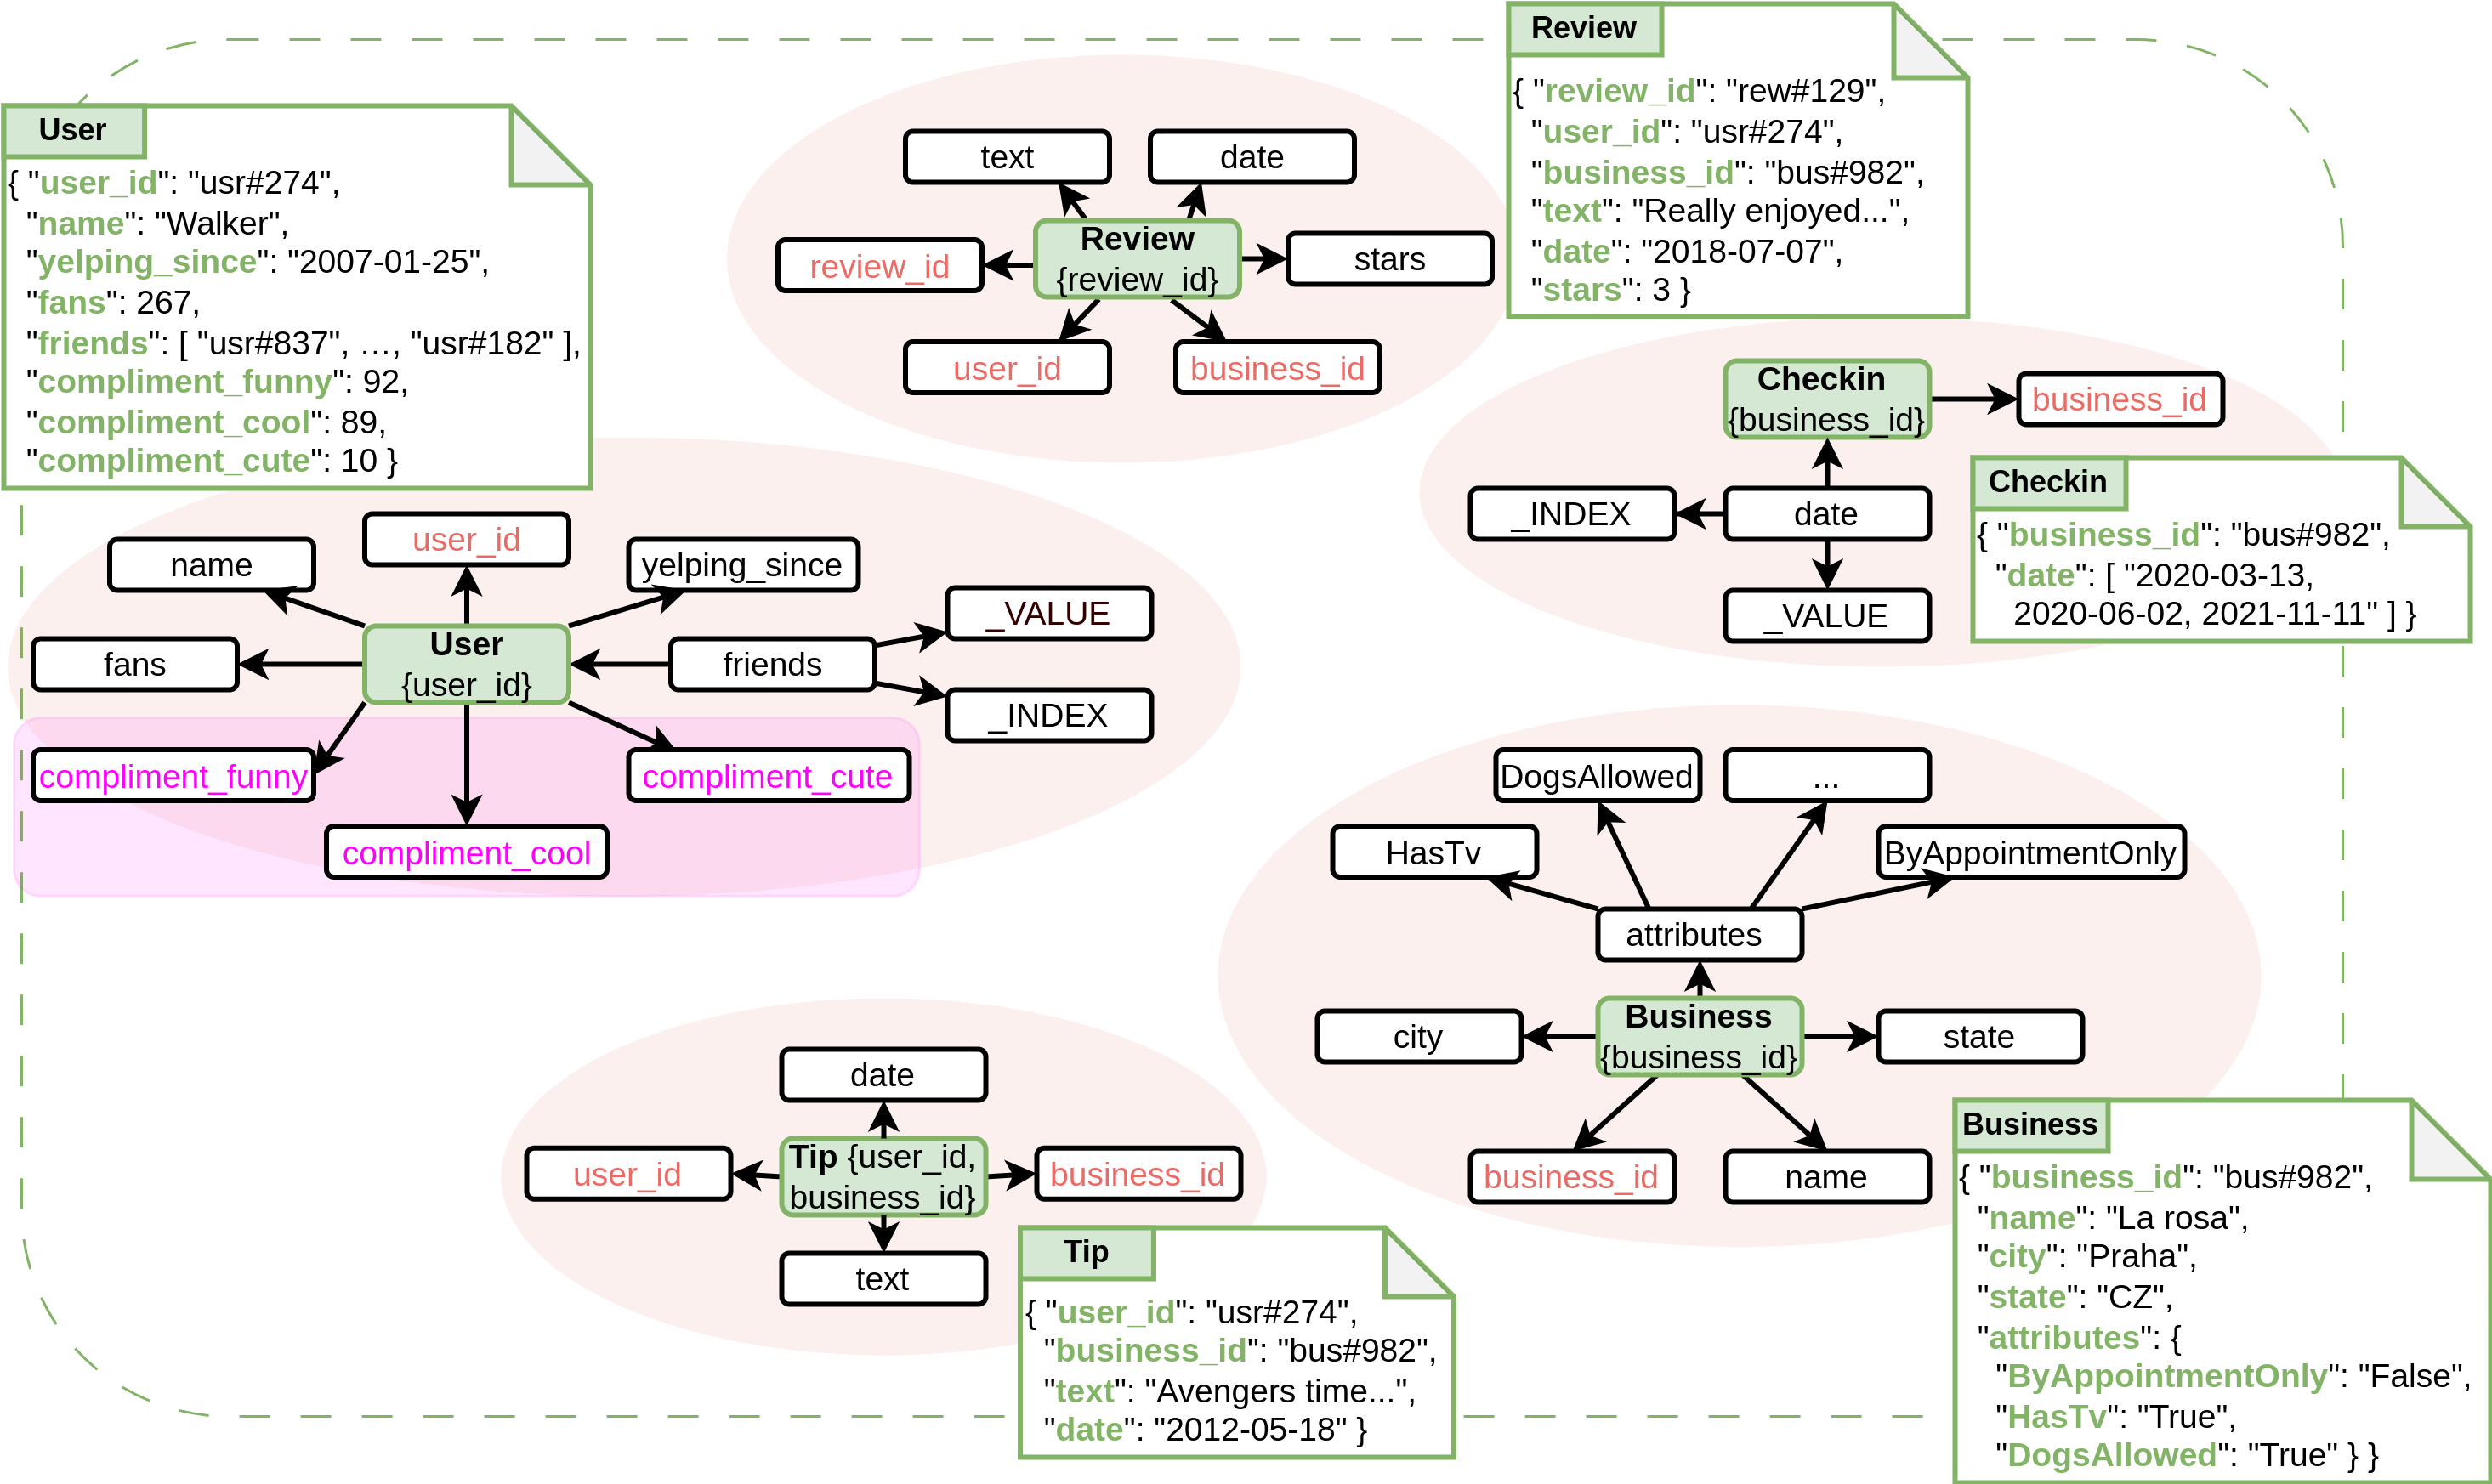
\includegraphics[width=\textwidth]{papers/enase_2025/figures/sk-initial.png}
    \caption{Input single-model JSON document collections and inferred initial schema category}
    \pLabel{fig:sk-initial}
\end{figure}

\begin{example}
Fig.~\pRef{fig:sk-edited} depicts the situation after the users visualized the initial schema category 
in \emph{MM-cat} 
and edited it 
using its extension \emph{MM-evocat} 
to solve the issues. \footnote{Some issues can be solved 
in \emph{MM-infer} 
(semi-)automatically, we use them just for illustration.} 
First, the users replaced repeating occurrences of properties \code{business\_id} and \code{user\_id} and expressed the references using the morphisms with the respective direction (the new morphisms are emphasized with dotted arrows). Second, the properties of kind \code{User} that are structurally and semantically equivalent were merged and transformed into a single property with a respective property \code{\_TYPE}.
\qed
\end{example}

\begin{figure}[ht!]
    \centering
    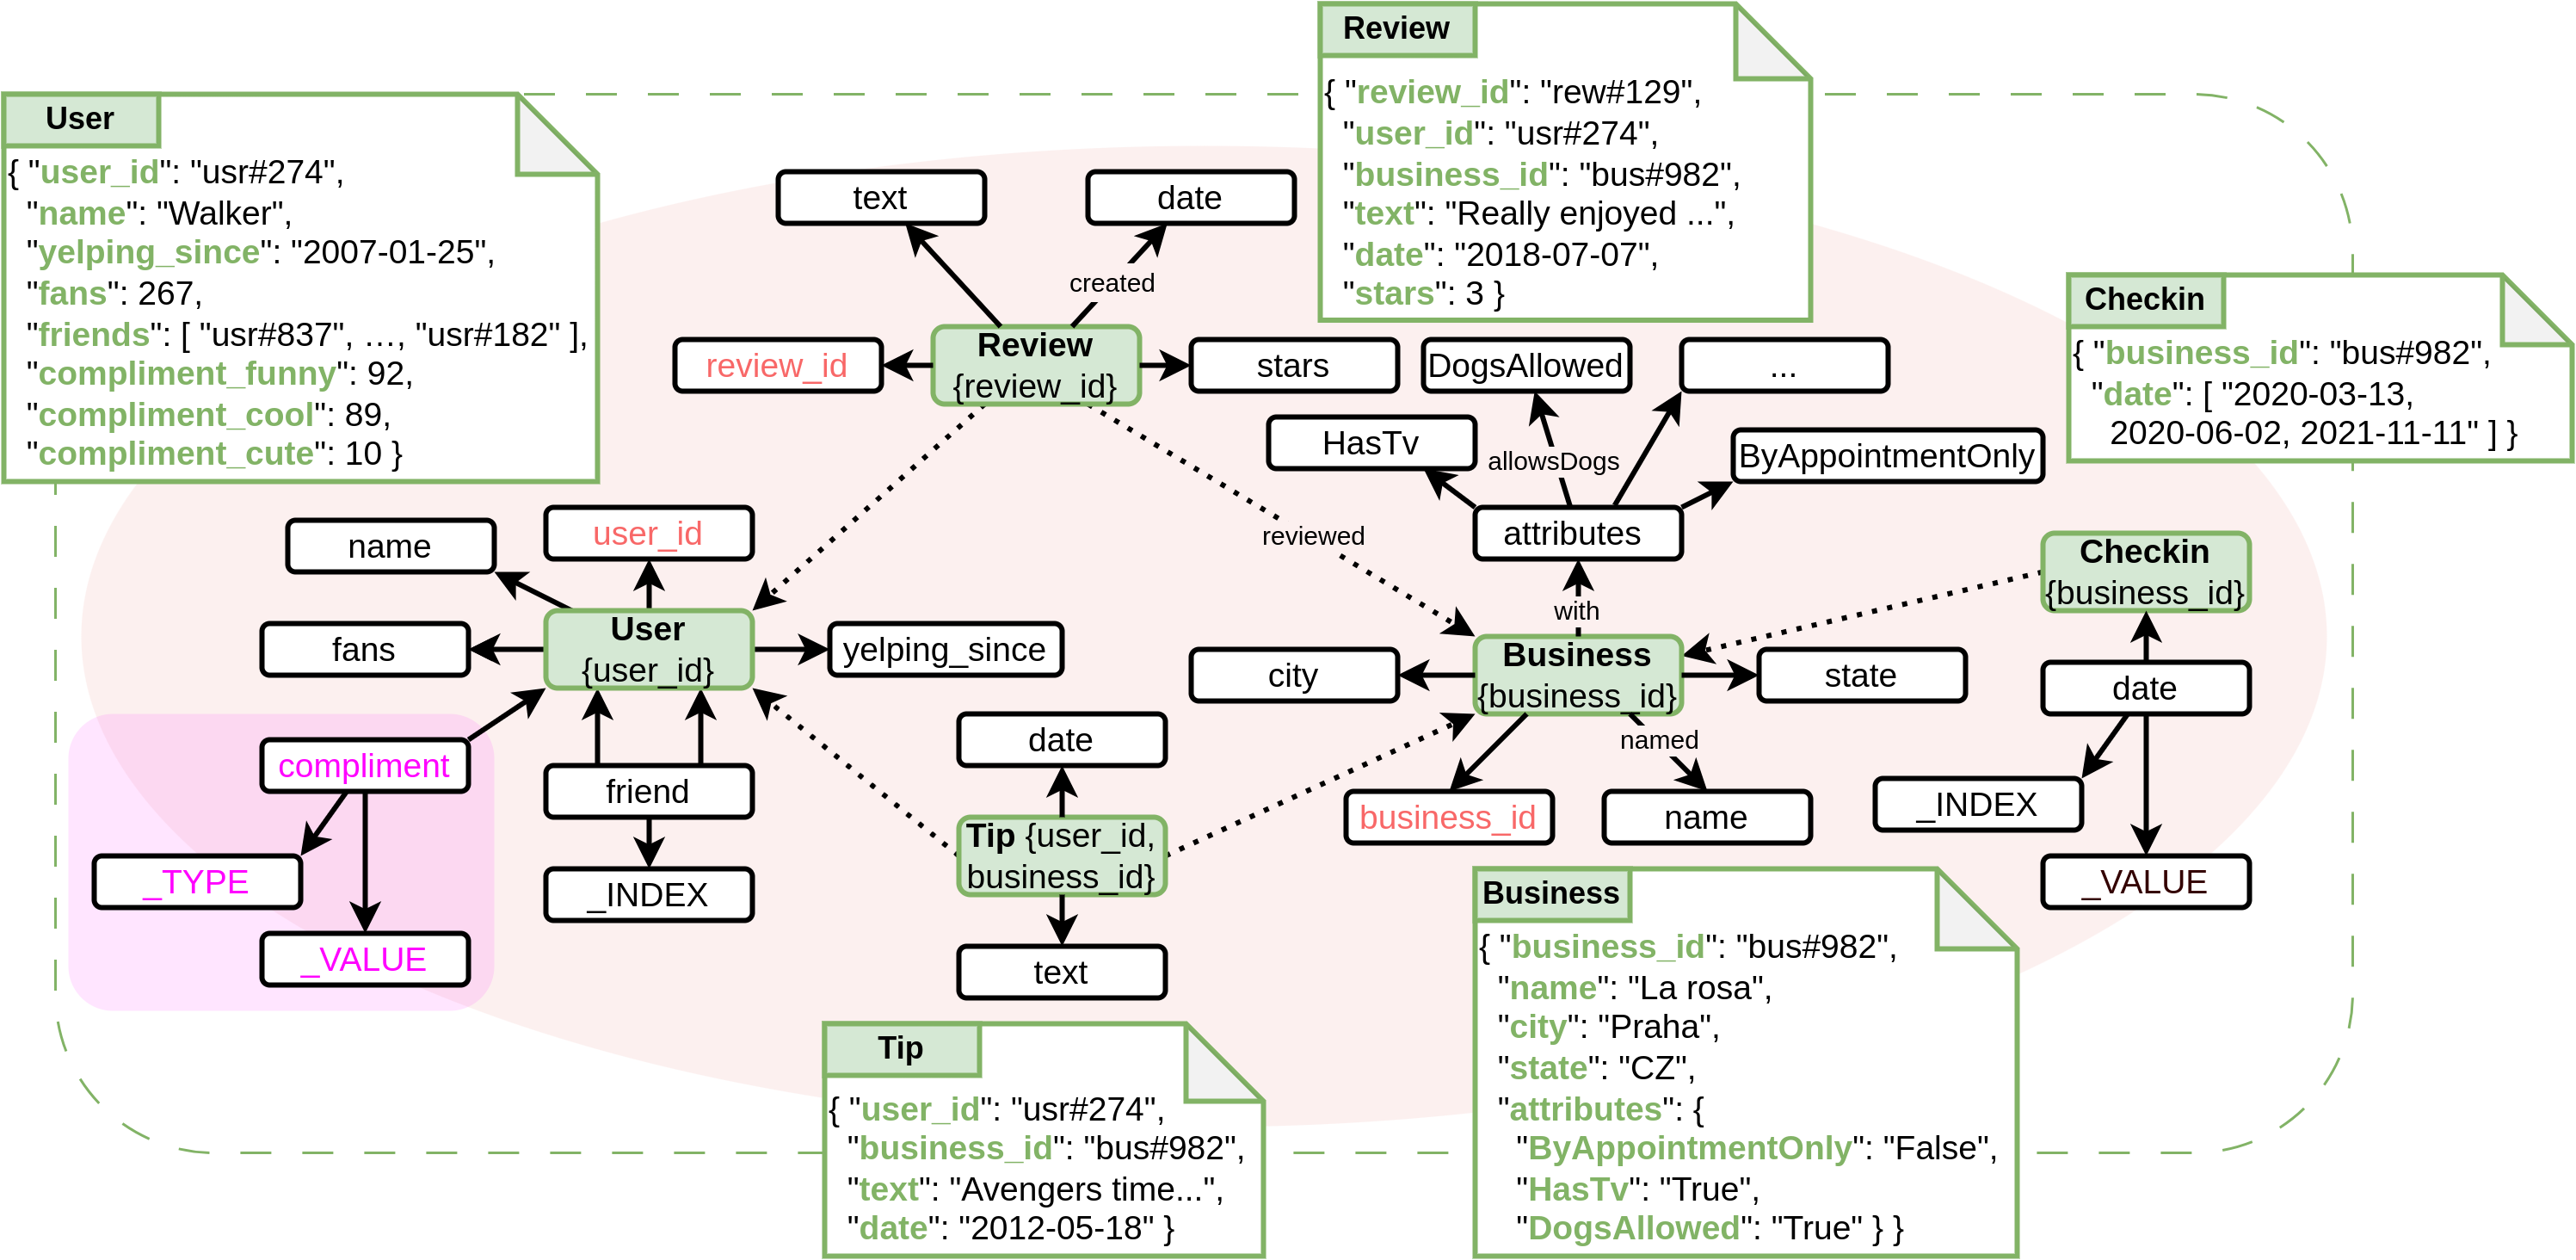
\includegraphics[width=\textwidth]{papers/enase_2025/figures/sk-edited.png}
    \caption{Edited (improved) schema category from Fig.~\pRef{fig:sk-initial}}
    \pLabel{fig:sk-edited}
\end{figure}


\begin{example}
Having the edited schema category, we can 
use \emph{MM-evocat} again to 
modify the mapping (initially to the input document model). Following \textbf{scenario~A}, we want to transform all the JSON document data into the relational model. The situation is depicted in Fig.~\pRef{fig:sk-mapping-3A}, where the users changed the mapping of the whole schema category to the relational model (violet). Namely, the original kinds \code{User}, \code{Review}, \code{Business}, and \code{Tip} were mapped to the respective relational tables instead of JSON collections. Regarding the features of the relational models, also the property \code{friend} of kind \code{User} and property \code{date} of kind \code{Checkin} had to be mapped to separate kinds \code{Friend} and \code{Date} (and, therefore, to respective separate relational tables). Similarly, the property \code{attribute} of kind \code{Business} was mapped to a map of attributes and thus a separate table.
\qed
\begin{figure}
    \centering
    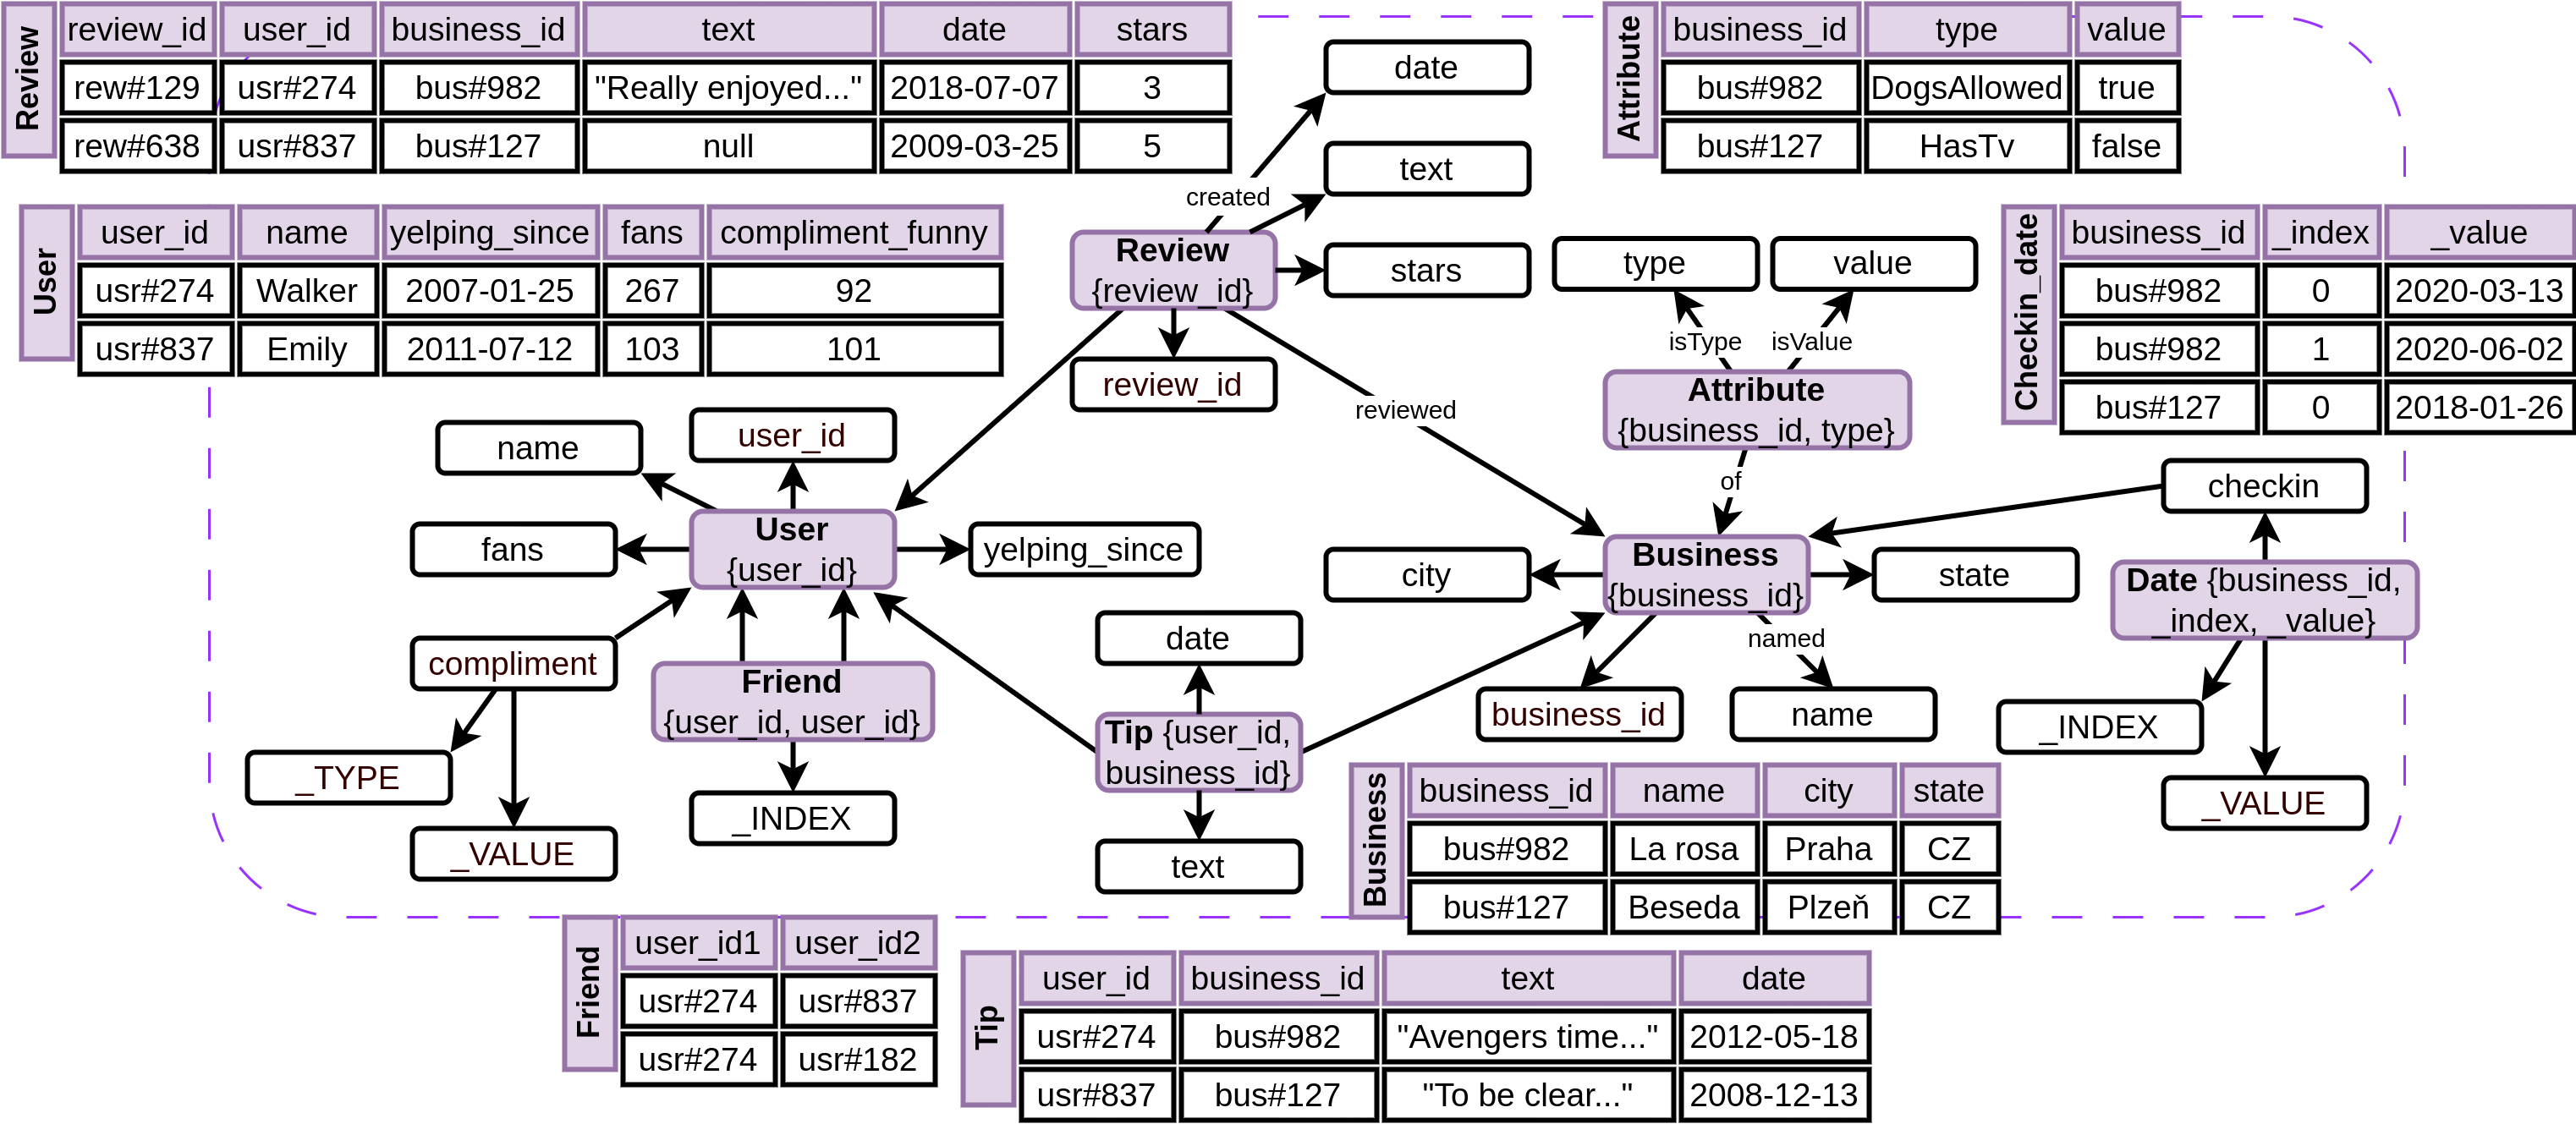
\includegraphics[width=\textwidth]{papers/enase_2025/figures/sk-mapping-3A.png}
    \caption{Schema category from Fig.~\pRef{fig:sk-edited} mapped to the relational model (scenario~A)}
    \pLabel{fig:sk-mapping-3A}
\end{figure}
\end{example}

\begin{example}
Following \textbf{scenario~B}, the users might find out that transforming all the data to the relational model is not optimal, and they decide to use the best of both worlds. As depicted in Fig.~\pRef{fig:sk-mapping-3B}, they kept the mapping of kinds \code{User} and \code{Friend} to the relational models, each to a separate table, like in Fig.~\pRef{fig:sk-mapping-3A}. They also want to keep a mapping of kinds \code{Review} and \code{Tip} to the relational model but to merge them into a single table because \code{Tip} is just a subset of \code{Review}. So, they create a new kind \code{Comment} that covers both of them and map it to a single table. The new kind requires property \code{comment\_id}, which we can reuse (for records of kind \code{Review}) or generate by a simple algorithm (for records of kind \code{Tip}).

Finally, they decided to embed the kinds \code{Attribute} and \code{Date}, which required separate relational tables, to the relational table of kind \code{Business}. So, they mapped them to the document model and embedded them to the kind \code{Business}. (Such a combination of models is supported, e.g., in PostgreSQL.) This transformation reduced the overhead of joining the same tables each time while keeping the kind \code{Business} mapped to the relational model. 

Fig.~\pRef{fig:sk-mapping-3B} depicts the result, where we get truly multi-model data represented in two logical models -- violet relational and green document.
\qed
\end{example}

\begin{figure}
    \centering
    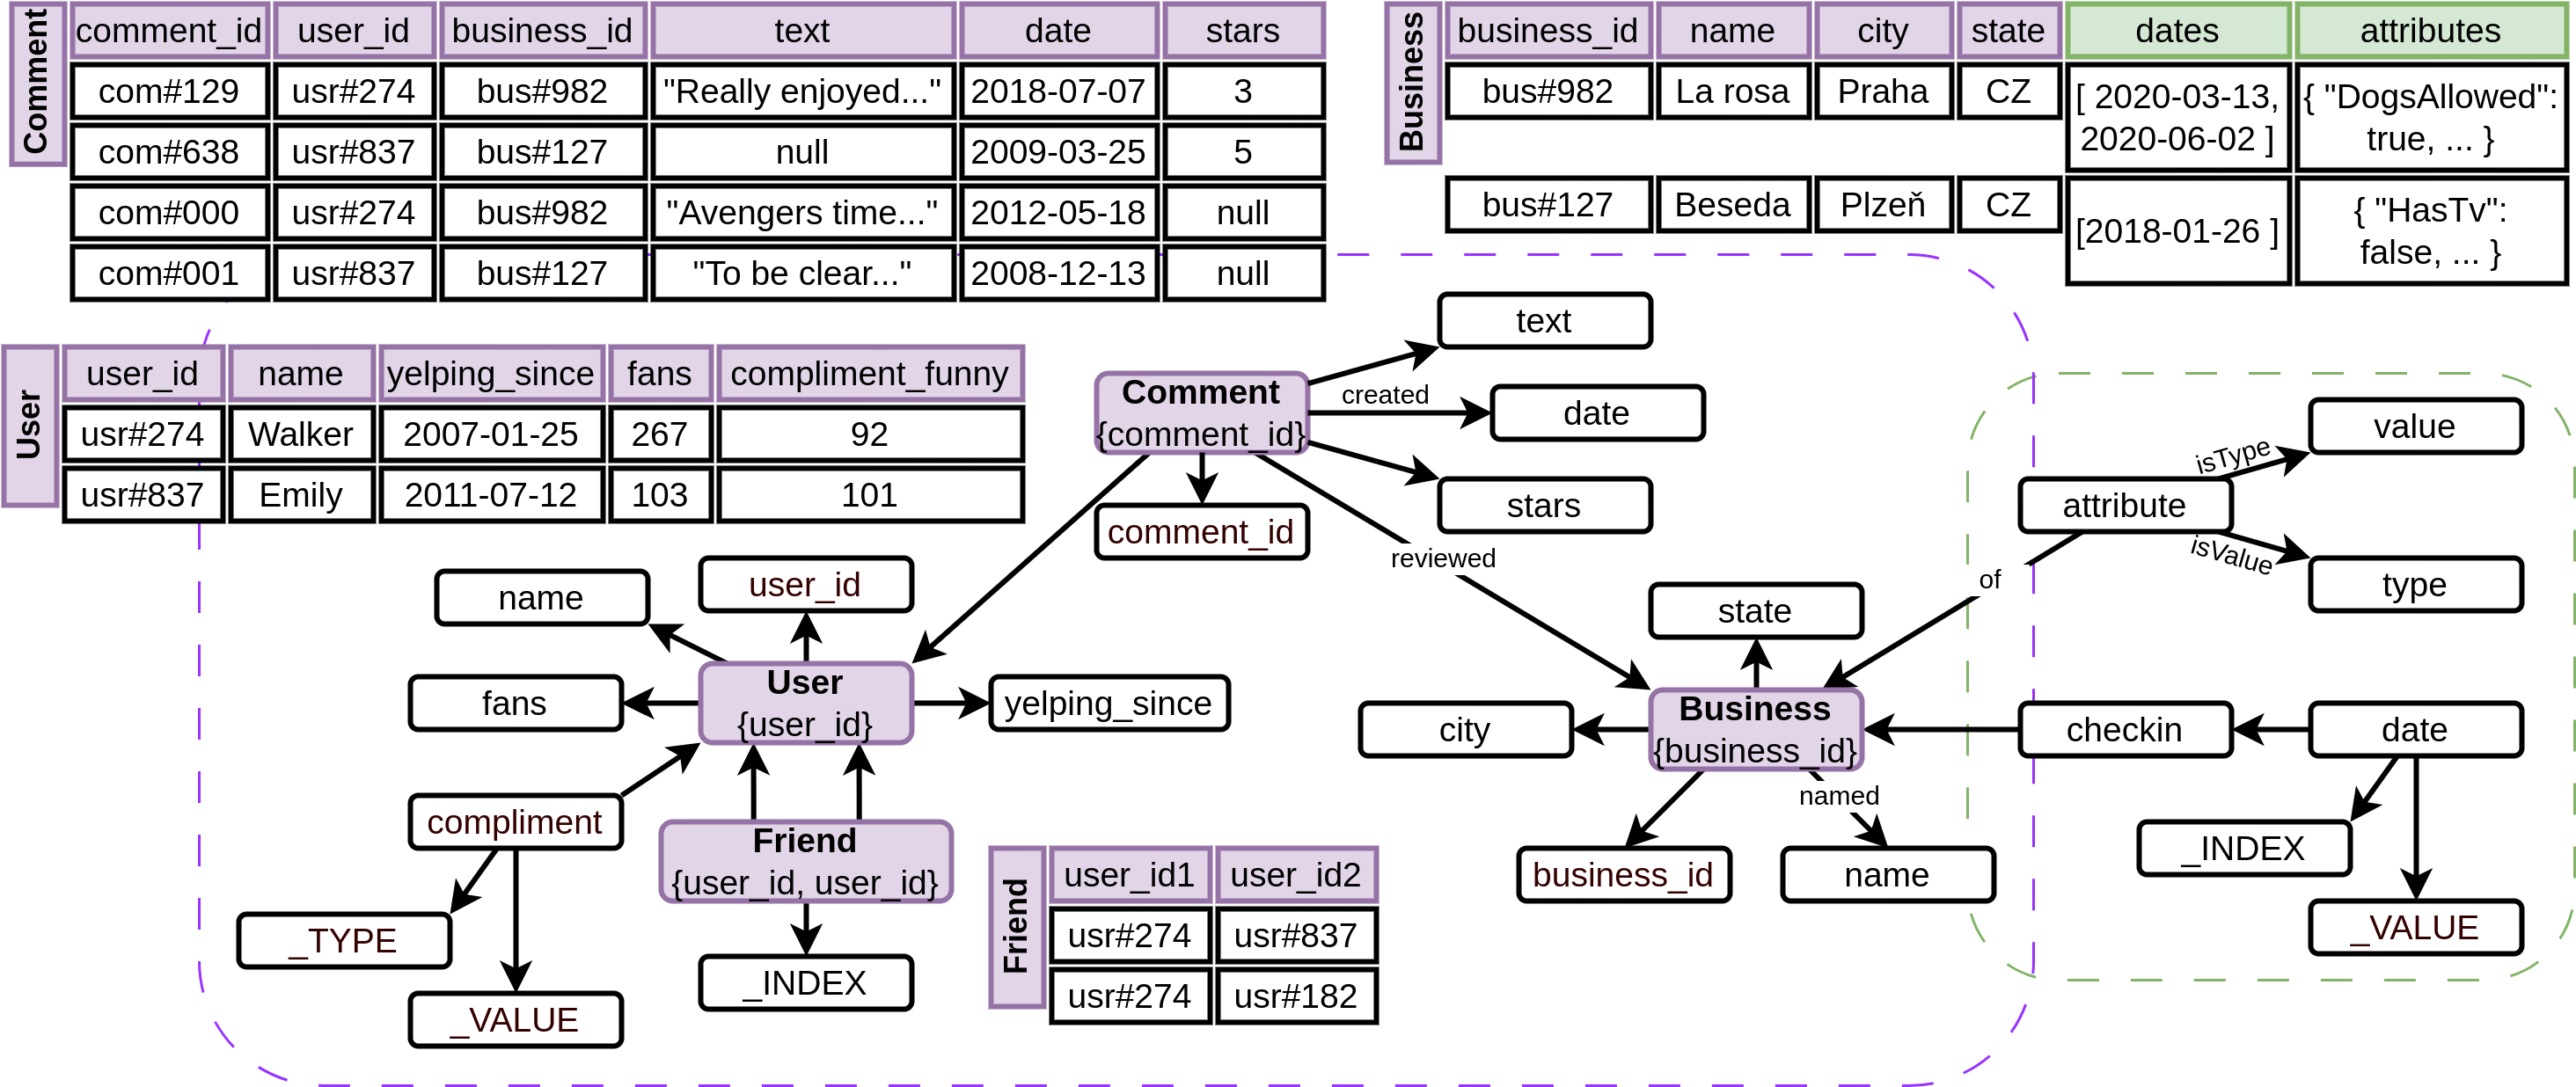
\includegraphics[width=\textwidth]{papers/enase_2025/figures/sk-mapping-3B.png}
    \caption{Schema category from Fig.~\pRef{fig:sk-edited} mapped to relational and document model  (scenario~B)}
    \pLabel{fig:sk-mapping-3B}
\end{figure}

\begin{example}
Finally, following \textbf{scenario~C} and as depicted in Fig.~\pRef{fig:sk-mapping-3C}, the users might further transform the multi-model data from a combination of two to a combination of three logical models and map the kind \code{Comment} to the wide-column model (red). This model is better suited for frequent data analysis, i.e., the type of queries the users might want to do with the comments. It also more naturally represents that tips do not have all the attributes of reviews.
\qed
\end{example}

\begin{figure}
    \centering
    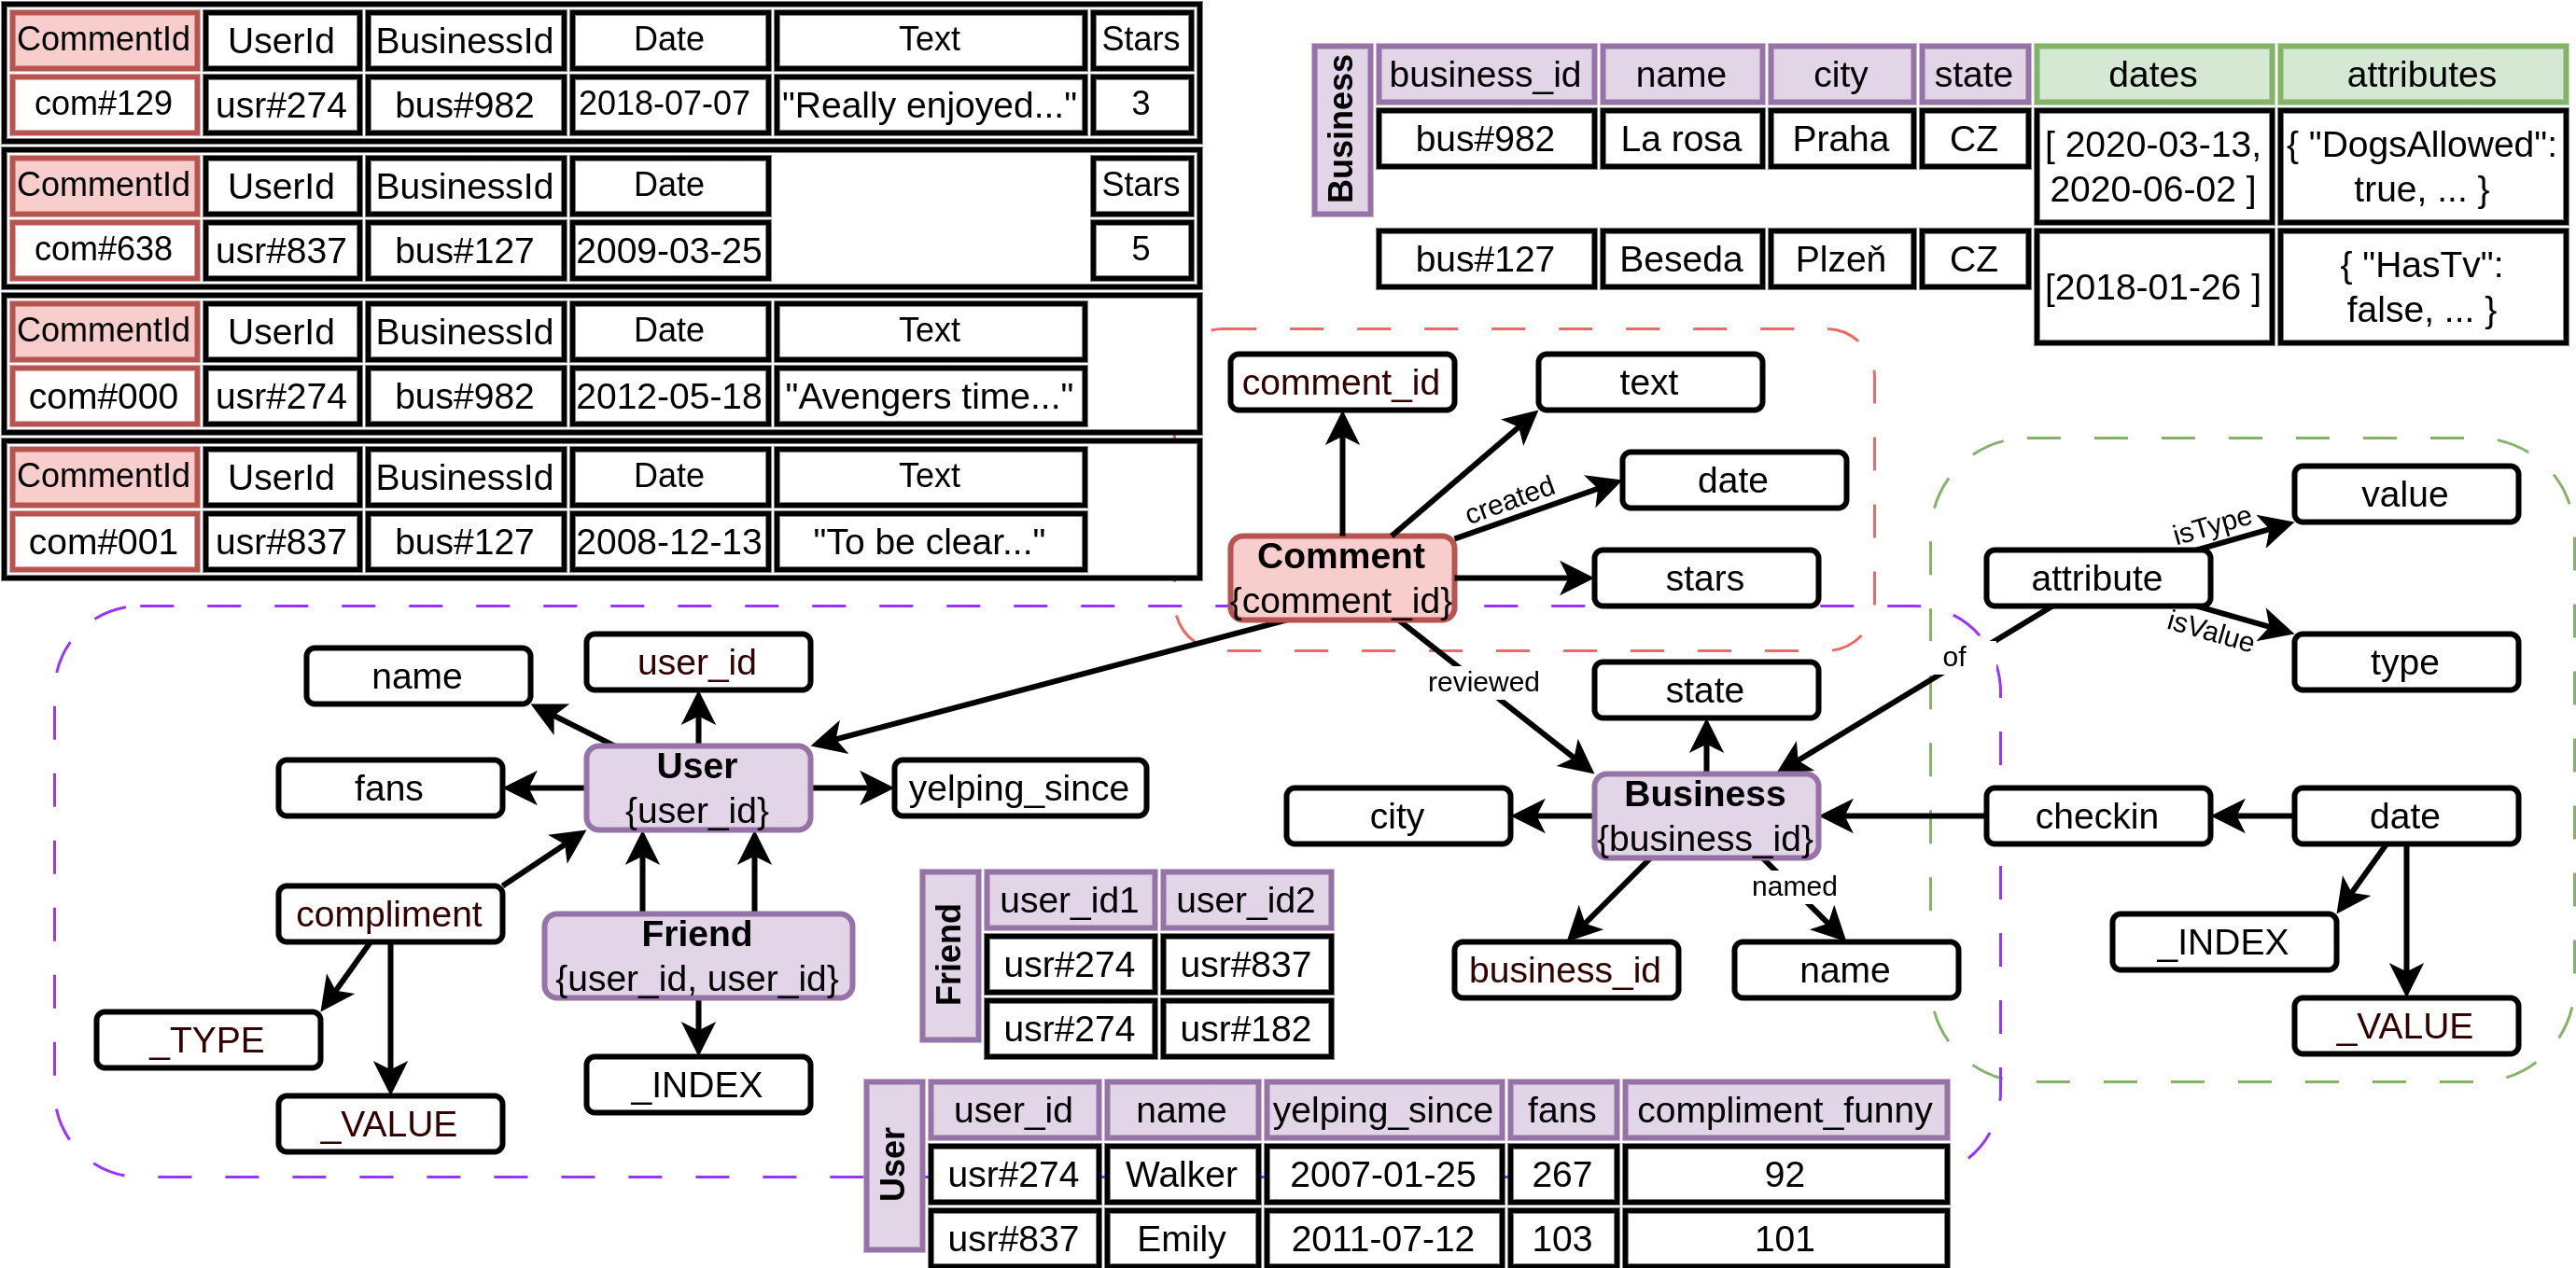
\includegraphics[width=\textwidth]{papers/enase_2025/figures/sk-mapping-3C.png}
    \caption{Schema category from Fig.~\pRef{fig:sk-mapping-3B} mapped to relational, document, and wide-column model  (scenario~C)}
    \pLabel{fig:sk-mapping-3C}
\end{figure}

So, as we can see, by using the framework, it is very simple to transform the input data to any multi-model data only by modification of the schema category and its mapping to the logical models. Nevertheless, we may also want a similar functionality for the queries. Extending the framework further 
with \emph{MM-quecat}
makes it possible to query over the schema category using MMQL~\citep{koupil2023universal}, a graph query language utilizing the SPARQL notation to query over the schema category. Depending on the specified mapping of the schema category to the logical models, the MMQL query can be translated 
using \emph{MM-quecat}
to be evaluated in the underlying DBMS. But, for our purposes, instead of querying, we only retrieve the query with the transformed data and use it for benchmarking. 

\begin{example}
For example, the users may want to query for \uv{\emph{names of businesses which have been reviewed since January 1st, 2023 and allow dogs}}. Its expression in MMQL over the improved schema category in Fig.~\pRef{fig:sk-edited} is provided in Fig.~\pRef{fig:query-mmql-1}. 
If the input data in Fig.~\pRef{fig:sk-edited} were stored in MongoDB\footnote{\url{https://www.mongodb.com/}}, its translation to MongoDB QL is provided in Fig.~\pRef{fig:query-mongo}. 
\qed
\end{example}

\begin{figure}[!htb]
    \begin{lstlisting}[language = MMQL]
        SELECT {
            ?business name ?name .
        }
        WHERE {
            ?business -reviewed/created ?date ;
                with/allowsDogs "true" ;
                named ?name .
            FILTER(?date > "2023-01-01")
        }
    \end{lstlisting}
    \caption{MMQL query over the improved schema category in Fig.~\pRef{fig:sk-edited}}\pLabel{fig:query-mmql-1}
\end{figure}

\begin{figure}[!htb]
    \begin{lstlisting}[language = MQL]
        db.review.aggregate([
            { $match: {
                date: { $gt: ISODate('2023-01-01') }
            } },
            { $lookup: {
                from: "business",
                localField: "business_id",
                foreignField: "business_id",
                as: "business"
            } },
            { $match: {
                attributes: { DogsAllowed: true }
            } },
            { $project: {
                _id: 0,
                name: "$business.name"
            } },
        ])
    \end{lstlisting}
    \caption{MongoDB QL query over data from Fig.~\pRef{fig:sk-edited}}\pLabel{fig:query-mongo}
\end{figure}

If we change the mapping to another model (or a combination of models) represented in another DBMS (or multiple DBMSs), we get the query expressed using the respective query language(s). In addition, if we change the part of the schema category accessed by the query, the modification of MMQL is ensured 
% !@# by \emph{MM-evoque} 
along with the modification of the mapping.

%An example is provided in the figure at the bottom left. 

\begin{example}
When we unify the business attributes to a map, as depicted in Fig.~\pRef{fig:sk-mapping-3A}, the MMQL query is modified to reflect the change, as depicted in Fig.~\pRef{fig:query-mmql-2}. In addition, in Fig.~\pRef{fig:sk-mapping-3A}, we also changed the mapping to the relational model (\textbf{scenario~A}). Assuming that now the data is stored in PostgreSQL, the respective mapping to the relational model ensures the translation of MMQL query to the SQL query provided in Fig.~\pRef{fig:query-sql}.
\qed
\end{example}

\begin{figure}[!htb]
    \begin{lstlisting}[language = MMQL]
        SELECT {
            ?business name ?name .
        }
        WHERE {
            ?business -reviewed/created ?date ;
                -of ?attribute ;
                named ?name .
            ?attribute isType "DogsAllowed" ;
                isValue "true" .
            FILTER(?date > "2023-01-01")
        }
    \end{lstlisting}
    \caption{MMQL query over schema category from Fig.~\pRef{fig:sk-mapping-3A}}\pLabel{fig:query-mmql-2}
\end{figure}

\begin{figure}[!htb]
    \begin{lstlisting}[language = SQL-fix]
        SELECT business.name AS name
        FROM business
        JOIN review ON business.business_id = review.business_id
        JOIN attribute ON business.business_id = attribute.business_id
        WHERE review.date > '2023-01-01'
            AND attribute.type = 'DogsAllowed'
            AND attribute.value = true
    \end{lstlisting}
    \caption{SQL query over data from Fig.~\pRef{fig:sk-mapping-3A} (scenario~A)}\pLabel{fig:query-sql}
\end{figure}

\begin{example}
If we use the combination of the document and relational model (\textbf{scenario~B}) depicted in Fig.~\pRef{fig:sk-mapping-3B}, we can assume that the data is still stored in PostgreSQL. As SQL in PostgreSQL is extended towards the support of cross-model queries over both relational and document data, i.e., SQL/JSON, the evaluation process again translates the MMQL query to a single, this time cross-model query, as depicted in Fig.~\pRef{fig:query-sql-json}. Note that despite the mapping change, the parts of the schema category accessed by the MMQL query remain untouched, so the MMQL query remains the same.
\qed
\end{example}

\begin{figure}[!htb]
    \begin{lstlisting}[language = SQL-fix]
        SELECT business.name AS name
        FROM business
        JOIN comment ON business.business_id = comment.business_id
        JOIN attribute ON business.business_id = attribute.business_id
        WHERE comment.date > '2023-01-01'
            AND attributes->>'DogsAllowed' = 'true'
    \end{lstlisting}
    \caption{SQL/JSON query over data from Fig.~\pRef{fig:sk-mapping-3B} (scenario~B)}\pLabel{fig:query-sql-json}
\end{figure}

\begin{example}
Finally, suppose we use a combination of models unsupported by a single multi-model DBMS (\textbf{scenario~C}) depicted in Fig.~\pRef{fig:sk-mapping-3C}. In that case, the evaluation consists of the decomposition of the query to two subqueries for the respective subsystems -- SQL for PostgreSQL and, e.g., CQL for Apache Cassandra\footnote{\url{https://cassandra.apache.org/}} -- as depicted in Fig.~\pRef{fig:query-cql-sql}. Thus, we can also test a family of DBMSs, together with the need to use an additional tool to merge the results. However, because the schema category did not change, the MMQL query stays the same again.
\qed
\end{example}

\begin{figure}[!htb]
    \begin{lstlisting}[language = SQL-fix]
        SELECT business_id
        FROM comment
        WHERE date > '2023-01-01'
    \end{lstlisting}
    
    \begin{lstlisting}[language = SQL-fix]
        SELECT name AS name
        FROM business
        WHERE business_id IN (/* CQL query result */)
            AND attributes->>'DogsAllowed' = 'true'
    \end{lstlisting}
    \caption{CQL and SQL queries over data from Fig.~\pRef{fig:sk-mapping-3C} (scenario~C)}\pLabel{fig:query-cql-sql}
\end{figure}


\subsection{Architecture}
Fig.~\pRef{fig:arch} provides the schema of the architecture of the proposed framework. In general, we utilize selected parts of the functionality of the existing and verified tools, extend them, integrate them, and roof the whole framework with a GUI to create the target framework. The expected work with the framework is as follows:

\begin{enumerate}
    \item The users provide the input single-model data to be transformed. The data can be stored in one of the supported DBMSs or provided in files. 
    \item \emph{MM-infer} parses the data and infers a schema that a new schema conversion module transforms to the initial schema category. % !@# The schema category is visualized using \emph{MM-cat}.
    \item The users can modify the schema category depending on their requirements. 
    % !@# Using its extension \emph{MM-evocat}
    The users can change the mapping of the schema category to selected combinations of logical models, or they can also change the structure of the schema category itself. When the modification is finished, \emph{MM-evocat} transforms the data according to the new mapping. 
    \item In addition, % !@# using \emph{MM-quecat}, 
    the users can specify an MMQL query, which is updated using \emph{MM-evoque} according to the changes in the mapping or the schema category to reflect the changes. 
\end{enumerate}


\begin{figure}[ht]
    \centering
    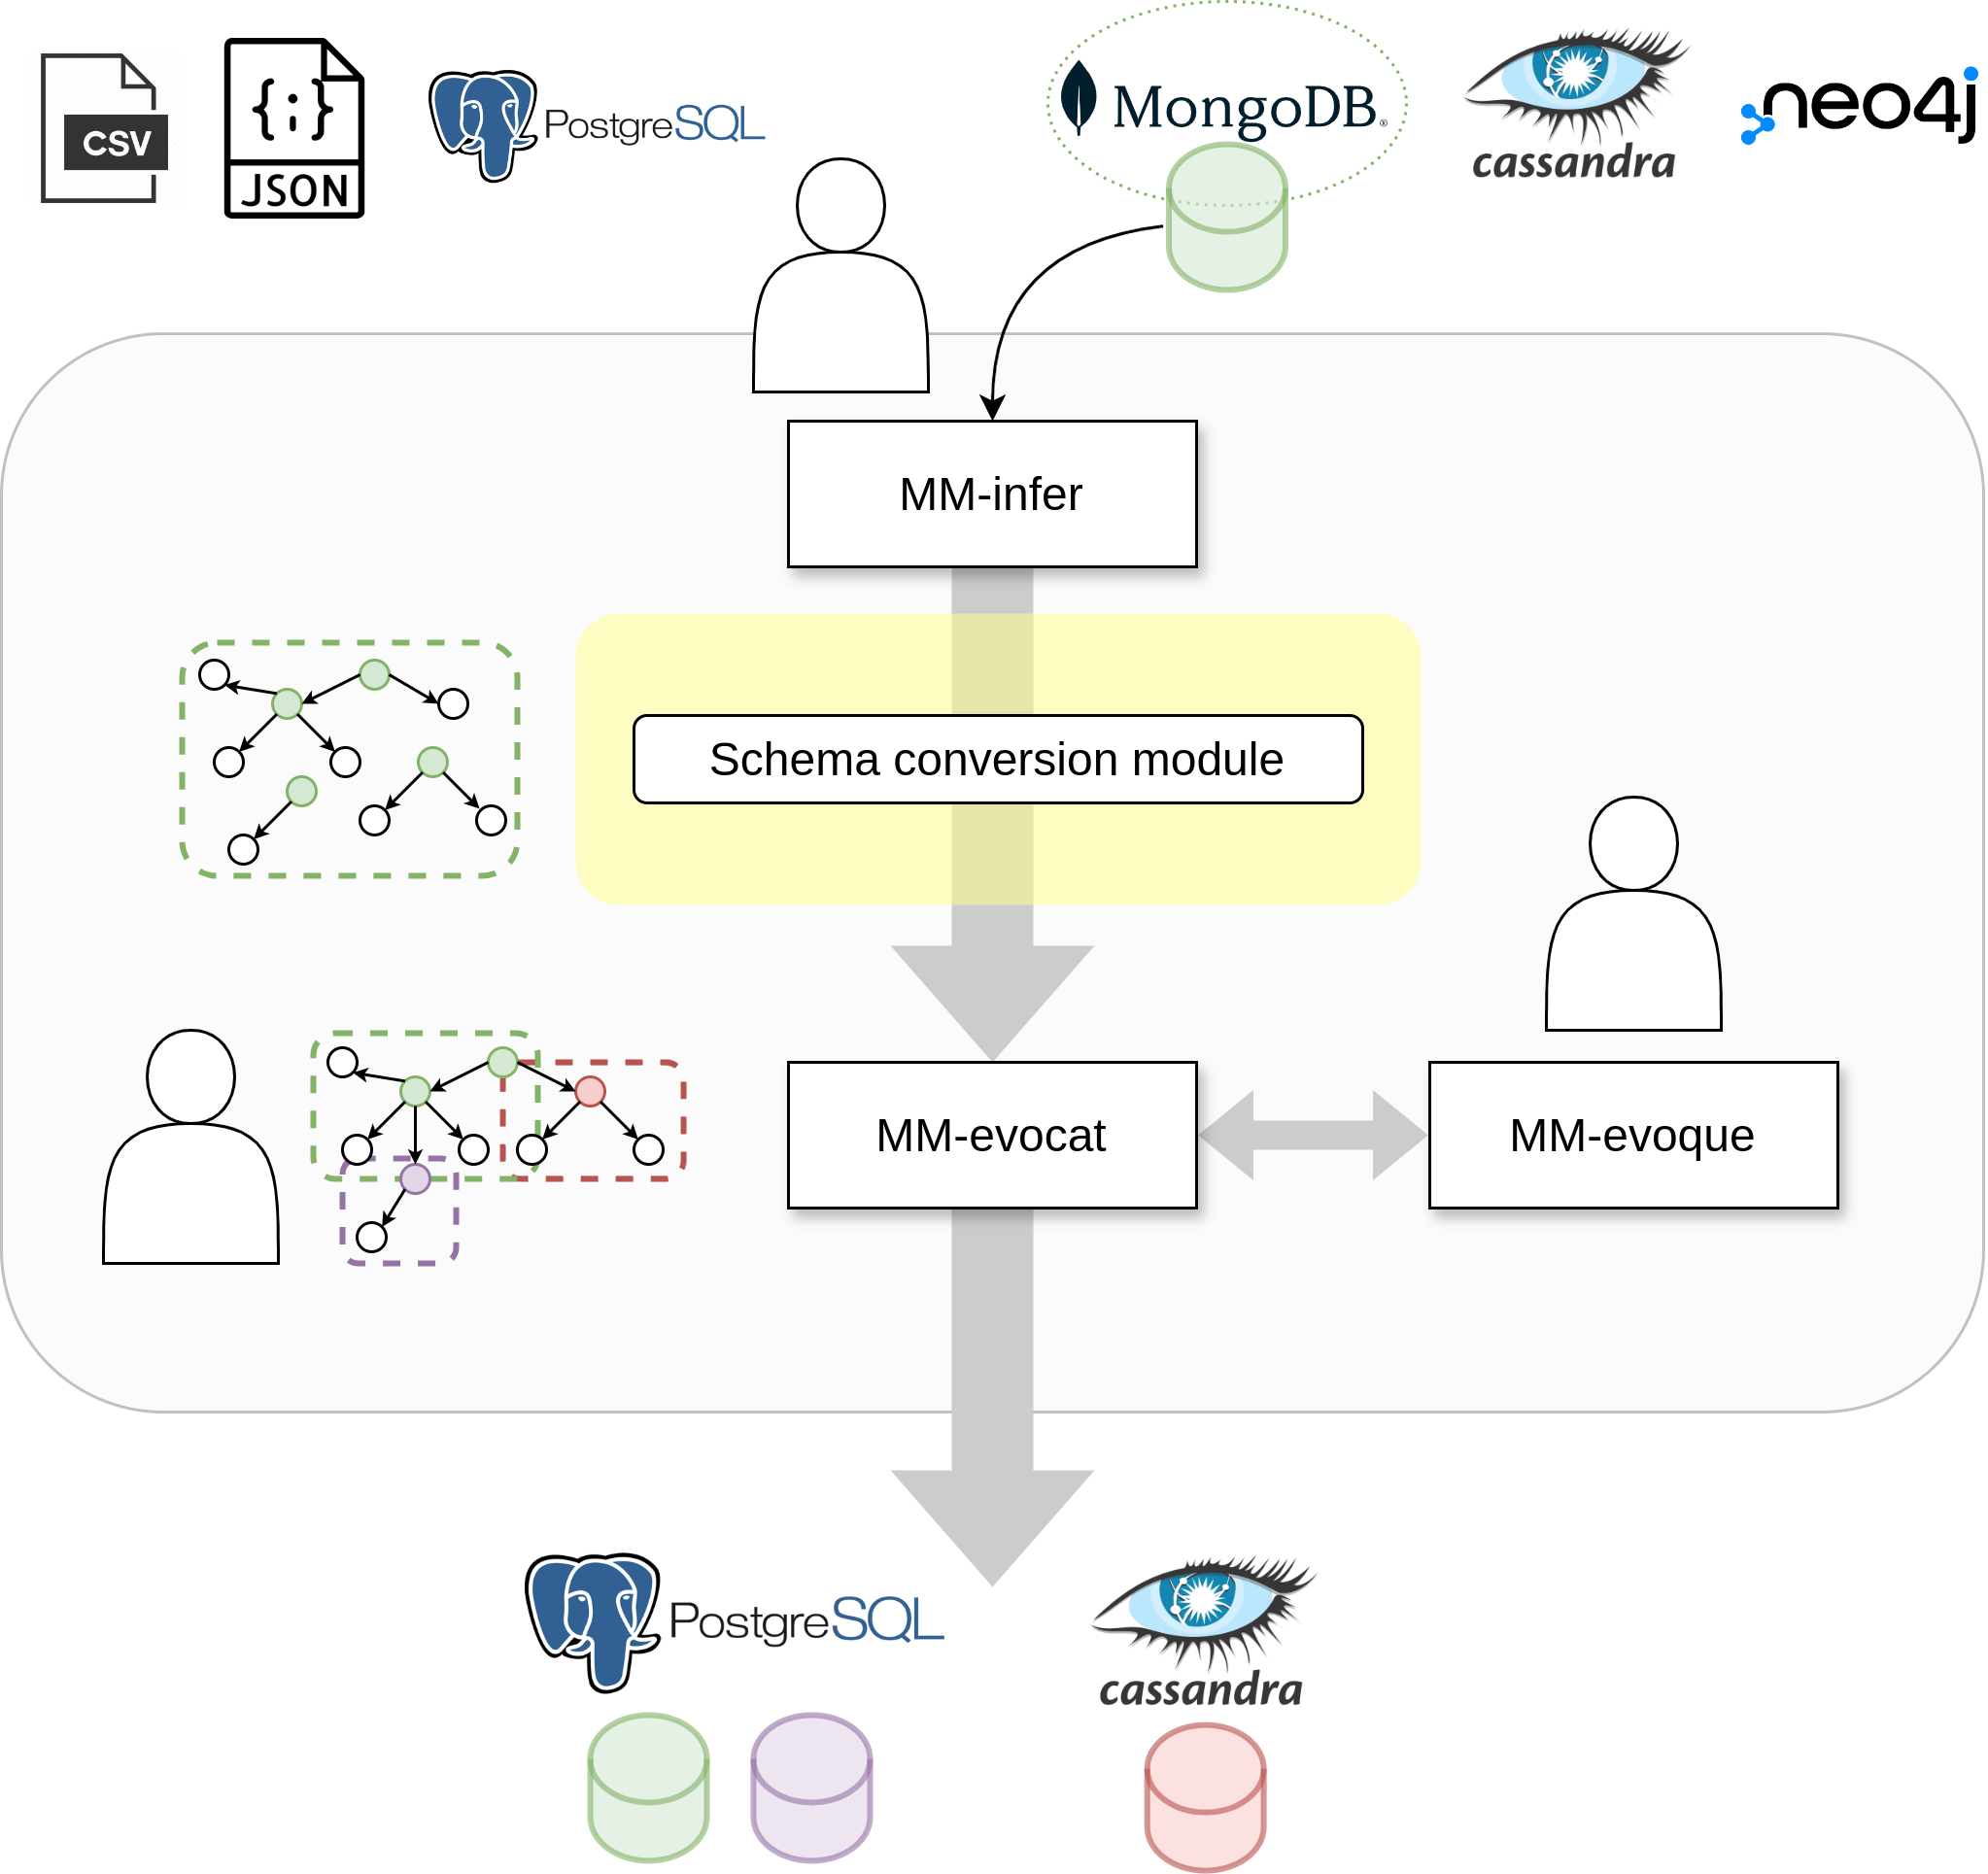
\includegraphics[width=\columnwidth]{papers/enase_2025/figures/dataFlow.png}
    \caption{Architecture of the framework}
    \pLabel{fig:arch}
\end{figure}


\subsection{Evaluation of the Proposed Solution}
Table~\pRef{tab:comparison} provides an overview of the advantages of framework utilization compared to manual data/query transformation. On average, depending on the complexity of the data, it is much faster. The framework enables us to infer the initial schema category and, thus, get the overall view of the data structure quickly. Also, all special cases and outliers are immediately provided to the users in a visual form. Also, the specification of the requested output is fast, and the transformation is performed automatically without the need to know the specific features of the underlying systems. 

Of course, we assume the framework supports all the required systems for which we want to create the testing data. However, integrating a new DBMS is simple, as it only requires implementing a respective wrapper. 
Once we have it, we do not need to implement any transformation script, and we can express the modification only by interacting with the framework tools.
Consequently, we avoid numerous user-defined errors, as the users are shielded from the technical details. Thus, we do not require an expert familiar with the specifics of various DBMSs.

The flexibility of the framework compared to manual data transformation is not limited. As mentioned above, although the framework currently supports MongoDB, PostgreSQL, neo4j, Apache Cassandra, JSON files, or CSV files, new DBMSs and data formats can be easily added using wrappers.

\begin{table*}
    \footnotesize
    \caption{Comparison of approaches using different metrics}
    \pLabel{tab:comparison}
    \centering
    %\begin{tabular}{|p{3cm}|p{2.5cm}|p{2cm}|}
    \begin{tabular}{|l|l|l|}
      \hline
      \bf Metric & \bf Without framework & \bf Using framework \\
      \hline            
      \hline
      \bf Time Required (hours)  & 10+ (estimation) & 0.5 (estimation) \\
      \hline
      \bf Lines of Code  & 200+ & 0 \\
      \hline
      \bf Potential for Errors  & \makecell[l]{High (coding, \\ manual transformation)} & Low (tool has been tested) \\
      \hline
      %\bf Learning Curve (hours)  & ?? & 1 \\
      %\hline
      \bf User Expertise Required  & Advanced & Beginner / Intermediate\\
      \hline
      \bf Flexibility / Customization  & High & High \\
      \hline
    \end{tabular}    
\end{table*}

Finally, Table~\pRef{tab:experiments} %provides an estimated number of operations needed for the three scenarios and the Yelp data set described in the running example. As we can see ...
illustrates the time required for user interactions across scenarios A, B, and C depicted in Figs.~\pRef{fig:sk-mapping-3A},~\pRef{fig:sk-mapping-3B}, and~\pRef{fig:sk-mapping-3C} when processing the Yelp dataset, comparing the conventional manual approach versus using the proposed framework tool. The framework streamlines the workflow by automating every step of the process. In Step~1, it infers the schema from the data. Following this, the framework facilitates editing the schema in Step~2 by providing a user-friendly interface that allows users to make necessary adjustments with minimal effort. In Step~3, it supports creating custom mappings between different data models. It then moves on to generate multi-model data in Step~4. Finally, it translates queries to operate across different data models in Step~5. The results demonstrate a substantial reduction in the time required for each step when using the framework, highlighting its efficiency and effectiveness in reducing user input and eventual~errors.

\begin{table*}
    \footnotesize
    \caption{User interaction needed in particular scenarios for the Yelp dataset}
    \pLabel{tab:experiments}
    \centering
    %\begin{tabular}{|c|p{1.4cm}|p{1.4cm}|p{1.4cm}|p{1.5cm}|}
    \begin{tabular}{|c|c|c|c|c|}
      \hline
      \textbf{Scenario} & \textbf{Step} & \bf \makecell{Without \\ framework (min)} & \bf \makecell{Using \\ framework (min)} & \bf Difference (min)  \\
      \hline
      \hline
      \multirow{5}{*}{A} & \multicolumn{1}{c|}{Step 1} & \multicolumn{1}{c|}{120} & \multicolumn{1}{c|}{5} & \multicolumn{1}{c|}{+115} \\\cline{2-5}
                         & \multicolumn{1}{c|}{Step 2} & \multicolumn{1}{c|}{120} & \multicolumn{1}{c|}{10} & \multicolumn{1}{c|}{+110} \\\cline{2-5}
                         & \multicolumn{1}{c|}{Step 3} & \multicolumn{1}{c|}{120} & \multicolumn{1}{c|}{12} & \multicolumn{1}{c|}{+108} \\\cline{2-5}
                         & \multicolumn{1}{c|}{Step 4} & \multicolumn{1}{c|}{180} & \multicolumn{1}{c|}{2} & \multicolumn{1}{c|}{+180} \\\cline{2-5}
                         & \multicolumn{1}{c|}{Step 5} & \multicolumn{1}{c|}{180} & \multicolumn{1}{c|}{0} & \multicolumn{1}{c|}{+180} \\\hline
      \multirow{3}{*}{B} & \multicolumn{1}{c|}{Step 3} & \multicolumn{1}{c|}{180} & \multicolumn{1}{c|}{12} & \multicolumn{1}{c|}{+168} \\\cline{2-5}
                         & \multicolumn{1}{c|}{Step 4} & \multicolumn{1}{c|}{240} & \multicolumn{1}{c|}{2} & \multicolumn{1}{c|}{+238} \\\cline{2-5}
                         & \multicolumn{1}{c|}{Step 5} & \multicolumn{1}{c|}{240} & \multicolumn{1}{c|}{0} & \multicolumn{1}{c|}{+240} \\\hline
      \multirow{3}{*}{C} & \multicolumn{1}{c|}{Step 3} & \multicolumn{1}{c|}{240} & \multicolumn{1}{c|}{16} & \multicolumn{1}{c|}{+234} \\\cline{2-5}
                         & \multicolumn{1}{c|}{Step 4} & \multicolumn{1}{c|}{300} & \multicolumn{1}{c|}{2} & \multicolumn{1}{c|}{+298} \\\cline{2-5}
                         & \multicolumn{1}{c|}{Step 5} & \multicolumn{1}{c|}{300} & \multicolumn{1}{c|}{0} & \multicolumn{1}{c|}{+300} \\\hline
    \end{tabular}
\end{table*}

%%%%%%%%%%%%%%%%%%%%%%%%%%%%%%%%%%%%%%%%%%%%%%%%%%%%
\section{Conclusion}
\pLabel{sec:concl}
This paper proposes a solution to the problem of lack of real-world multi-model data (and the respective queries). We use a different approach instead of the common strategy of generating a synthetic dataset despite having numerous realistic features. Using a specific utilization of our previously created toolset, we introduce the idea of a transformation framework that can transform a given, preferably real-world, dataset into a preferred multi-model dataset. Using a well-known dataset, Yelp, we demonstrate the advantages and applicability of the idea.

Our future work will focus primarily on implementing a common interface that will cover the whole functionality of the proposed framework and simplify the integration of the tools. In addition, we want to focus on the \textit{simulation of the evolution} of the resulting datasets, either through user specification or through the detection of changes in the input single-model data or operations. Lastly, we want to create a \textit{repository of the resulting multi-model datasets} to provide a robust source of test cases to be immediately used. We also want to perform \textit{extensive experiments with the datasets} to provide unbiased benchmarking results for elected multi-model databases.




%%%%%%%%%%%%%%%%%%%%%%%%%%%%%%%%%%%%%%%%%%%%%%%%%%%%
% \section*{Acknowledgment}
% This work was supported by the GAČR grant no. 23-07781S and GAUK grant no. 292323.
